%%%%%%%%%%%%%%%%%%%%%%%%%%%%%%%%%%%%%%%%%%%%%%%%%%%%%%%%%%%%
% ATTENTION !!!!!
% Ne pas écrire ici, ce fichier est fait pour la mise en page
% Pour écrire, éditer le fichier portant le nom de la partie 
%%%%%%%%%%%%%%%%%%%%%%%%%%%%%%%%%%%%%%%%%%%%%%%%%%%%%%%%%%%%

%%%% Packages utilisés pour ce rapport
\documentclass[12pt,openany]{report} %taille de police et type de document
\usepackage[utf8]{inputenc} % type d'encodage
\usepackage[francais]{babel} % pour le respect des règles typographique française
\usepackage{lmodern} % paquet de police (ressemble à time new roman) 

\usepackage{fullpage} % pour gérer les tailles de marges
\usepackage{fancyhdr} % pour plus d'option de mise en page
\usepackage{titlesec} % permet de gérer la mise en page des titres
\usepackage{hyperref} % pour avoir des lien hypertexte
\usepackage{setspace} % pour l'espace interligne

\usepackage{gensymb} % 3 paquets pour les expression mathématiques
\usepackage{amsmath}
\usepackage{amssymb}

\usepackage{tocloft} % pour les tables de matières, de figures et de tableaux
\usepackage{graphicx} % pour inclure des images
\usepackage{caption} % pour les légendes
\usepackage{listingsutf8} % pour l'ajout de code

\usepackage{multicol} % pour écrire du texte dans plusieurs colonnes
\usepackage{minitoc} % pour plus d'option de mise en page

\usepackage[toc,page]{appendix}
\usepackage{cleveref}


\pagestyle{fancy}
\lhead{}
\chead{}
\rhead{}
\lfoot{}
\cfoot{}
\rfoot{\thepage}
\renewcommand{\headrulewidth}{0pt}
\renewcommand{\footrulewidth}{0pt}

\fancypagestyle{plain}{
\lhead{}
\chead{}
\rhead{}
\lfoot{}
\cfoot{}
\rfoot{\thepage}
\renewcommand{\headrulewidth}{0pt}
\renewcommand{\footrulewidth}{0pt}
}

\onehalfspacing

%titre, auteur, date
\title{Introduction à l'utilisation d'un système GNU/LINUX}
\author{Nicolas Cubric\\Association Robotronik Phelma}
%\date{}

% début du document
\begin{document}
%Formattage des titres de chapitre, section, sous-section
\titleformat{\chapter}[block]{\bf\huge}{\thechapter}{2pc}{}   
\titlespacing*{\chapter}{0pt}{-30pt}{15pt}
\renewcommand\thechapter{\Roman{chapter}}

\titleformat{\section}[block]{\bf\Large}{\thesection}{2pc}{}
\renewcommand\thesection{\thechapter.\arabic{section}}

\titleformat{\subsection}[block]{\bf\large}{\thesubsection}{2pc}{}
\renewcommand\thesubsection{\thesection.\arabic{subsection}}


%Formattage du titre du sommaire
\setlength{\cftbeforetoctitleskip}{-2em}

\makeatletter

% page de garde
\begin{titlepage}
\begin{center}
    
\includegraphics[width=0.3\textwidth]{Images/logoclub.jpg}
    
    \vfill
    
    {\large \textbf{}}\\
    \vspace*{1cm}
    {\LARGE\textbf{\@title}}
    
    \vfill
    
    
\includegraphics[width=0.5\textwidth]{Images/tux.png}
    
    \vfill
    
    {\large\emph{} \textbf{}}\\
    \vspace*{0.5cm}
    {\large\textbf{\@author}}\\
    
    \vfill
    
    {\large \@date}
\end{center}
\end{titlepage}

\include{Remerciements}

%Sommaire, tables des figures et des tableaux
\renewcommand{\contentsname}{Sommaire}
\tableofcontents
\clearpage

\listoffigures
\clearpage

\listoftables
\clearpage

\chapter{Linux c'est quoi ?}

Linux ou plus précisément GNU/Linux est un système d'exploitation basé sur un noyau UNIX. À la différence de Windows, qui est basé sur un noyau DOS, Linux est open source, c'est à dire que tout le monde peut avoir accès aux code sources et les modifiés à sa guise. La seule règle étant de laisser son œuvre libre et disponible à tous.


\chapter{L'arborescence}

L'arborescence sous Linux correspond à la manière sont agencés les dossiers (directory en anglais) les uns par rapport aux autres.

\begin{center}
	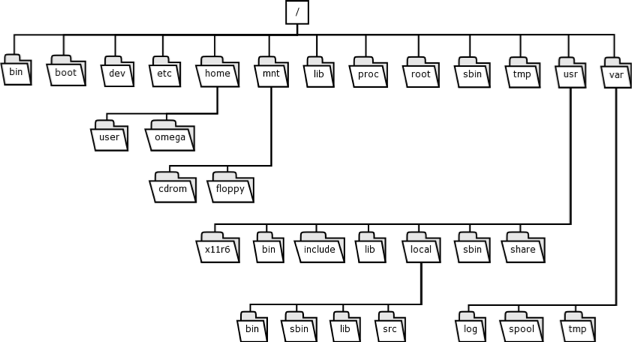
\includegraphics[width=0.7\textwidth]{Images/arborescence.png}
	\captionof{figure}{Arborescence d'un système GNU/Linux}
\end{center}

Vous l'aurez peut être remarqué mais tous les dossiers mènent à /. Ce dossier a pour petit nom, root. Il est ce que l'on appelle la racine du système. De ce dossier découle une floppé d'autre. Chacun à son utilité, nous allons voir les "plus important"
\begin{itemize}
	\item home : ce dossier contient les fichiers des utilisateurs. C'est ici que se situe les données des utilisateurs.
	\item 
\end{itemize}


% bibliographie
% \addcontentsline{toc}{chapter}{Bibliographie}
% \bibliographystyle{apalike}
% \bibliography{biblio.bib}
% % pour inserer des références pas citées dans le texte
\nocite{}

\end{document}

